%!TEX TS-program = xelatex
\documentclass[12pt, a4paper, oneside]{article}

% Можно вставить разную преамбулу
% пакеты для математики
\usepackage{amsmath,amsfonts,amssymb,amsthm,mathtools}  
\mathtoolsset{showonlyrefs=true}  % Показывать номера только у тех формул, на которые есть \eqref{} в тексте.

\usepackage[british,russian]{babel} % выбор языка для документа
\usepackage[utf8]{inputenc}          % utf8 кодировка

% Основные шрифты 
\usepackage{fontspec}         
\setmainfont{Linux Libertine O}  % задаёт основной шрифт документа

% Математические шрифты 
\usepackage{unicode-math}     
\setmathfont[math-style=upright]{euler.otf} 

\setmathfont[range={\mathbb, \mathop, \heartsuit, \angle, \smile, \varheartsuit}]{Asana-Math.otf}

%%%%%%%%%% Работа с картинками и таблицами %%%%%%%%%%
\usepackage{graphicx} % Для вставки рисунков                
\usepackage{graphics}
\graphicspath{{images/}{pictures/}}   % папки с картинками

\usepackage[figurename=Картинка]{caption}

\usepackage{wrapfig}    % обтекание рисунков и таблиц текстом

\usepackage{booktabs}   % таблицы как в годных книгах
\usepackage{tabularx}   % новые типы колонок
\usepackage{tabulary}   % и ещё новые типы колонок
\usepackage{float}      % возможность позиционировать объекты в нужном месте
\renewcommand{\arraystretch}{1.2}  % больше расстояние между строками


%%%%%%%%%% Графики и рисование %%%%%%%%%%
\usepackage{tikz, pgfplots}  % языки для графики
%\pgfplotsset{compat=1.16}

\usepackage{todonotes} % для вставки в документ заметок о том, что осталось сделать
% \todo{Здесь надо коэффициенты исправить}
% \missingfigure{Здесь будет Последний день Помпеи}
% \listoftodos --- печатает все поставленные \todo'шки

\usepackage{multicol}

%%%%%%%%%% Внешний вид страницы %%%%%%%%%%

\usepackage[paper=a4paper, top=20mm, bottom=15mm,left=20mm,right=15mm]{geometry}
\usepackage{indentfirst}    % установка отступа в первом абзаце главы

\usepackage{setspace}
\setstretch{1.15}  % межстрочный интервал
\setlength{\parskip}{4mm}   % Расстояние между абзацами
% Разные длины в LaTeX: https://en.wikibooks.org/wiki/LaTeX/Lengths

% свешиваем пунктуацию
% теперь знаки пунктуации могут вылезать за правую границу текста, при этом текст выглядит ровнее
\usepackage{microtype}

% \flushbottom                            % Эта команда заставляет LaTeX чуть растягивать строки, чтобы получить идеально прямоугольную страницу
\righthyphenmin=2                       % Разрешение переноса двух и более символов
\widowpenalty=300                     % Небольшое наказание за вдовствующую строку (одна строка абзаца на этой странице, остальное --- на следующей)
\clubpenalty=3000                     % Приличное наказание за сиротствующую строку (омерзительно висящая одинокая строка в начале страницы)
\tolerance=10000     % Ещё какое-то наказание.

% мои цвета https://www.artlebedev.ru/colors/
\definecolor{titleblue}{rgb}{0.2,0.4,0.6} 
\definecolor{blue}{rgb}{0.2,0.4,0.6} 
%\definecolor{red}{rgb}{1,0,0.2} 
\definecolor{green}{rgb}{0, 0.6, 0}
\definecolor{purp}{rgb}{0.4,0,0.8} 

\definecolor{red}{RGB}{213,94,0}
\definecolor{yellow}{RGB}{240,228,66}


% цвета из geogebra 
\definecolor{litebrown}{rgb}{0.6,0.2,0}
\definecolor{darkbrown}{rgb}{0.75,0.75,0.75}

% Гиперссылки
\usepackage{xcolor}   % разные цвета

\usepackage{hyperref}
\hypersetup{
	unicode=true,           % позволяет использовать юникодные символы
	colorlinks=true,       	% true - цветные ссылки
	urlcolor=blue,          % цвет ссылки на url
	linkcolor=black,          % внутренние ссылки
	citecolor=green,        % на библиографию
	breaklinks              % если ссылка не умещается в одну строку, разбивать её на две части?
}

% меняю оформление секций 
\usepackage{titlesec}
\usepackage{sectsty}

% меняю цвет на синий
\sectionfont{\color{titleblue}}
\subsectionfont{\color{titleblue}}

% кружочки у цифр в секциях
\renewcommand{\thesection}{\arabic{section}}

% https://ru.overleaf.com/learn/latex/Sections_and_chapters

% выбрасываю нумерацию страниц и колонтитулы 
%\pagestyle{empty}

% синие круглые бульпоинты в списках itemize 
\usepackage{enumitem}

\definecolor{itemizeblue}{rgb}{0, 0.45, 0.70}

\newcommand*{\MyPoint}{\tikz \draw [baseline, fill=itemizeblue, draw=blue] circle (2.5pt);}
\renewcommand{\labelitemi}{\MyPoint}

\AddEnumerateCounter{\asbuk}{\@asbuk}{\cyrm}
\renewcommand{\theenumi}{\asbuk{enumi}}

% расстояние в списках
\setlist[itemize]{parsep=0.4em,itemsep=0em,topsep=0ex}
\setlist[enumerate]{parsep=0.4em,itemsep=0em,topsep=0ex}

% эпиграфы
\usepackage{epigraph}
\setlength\epigraphwidth{.6\textwidth}
\setlength\epigraphrule{0pt}

%%%%%%%%%% Свои команды %%%%%%%%%%

% Математические операторы первой необходимости:
\DeclareMathOperator{\sgn}{sign}
\DeclareMathOperator*{\argmin}{arg\,min}
\DeclareMathOperator*{\argmax}{arg\,max}
\DeclareMathOperator{\Cov}{Cov}
\DeclareMathOperator{\Var}{Var}
\DeclareMathOperator{\Corr}{Corr}

\DeclareMathOperator{\Pois}{Pois}
\DeclareMathOperator{\Geom}{Geom}
\DeclareMathOperator{\Exp}{Exp}

%\DeclareMathOperator{\E}{\mathbb{E}}
\DeclareMathOperator{\Med}{Med}
\DeclareMathOperator{\Mod}{Mod}
\DeclareMathOperator*{\plim}{plim}

% команды пореже
\newcommand{\const}{\mathrm{const}}  % const прямым начертанием
\newcommand{\iid}{\sim i\,i\,d\,\,}  % ну вы поняли...
\newcommand{\fr}[2]{\ensuremath{^{#1}/_{#2}}}   % особая дробь
\newcommand{\ind}[1]{\mathbbm{1}_{\{#1\}}} % Индикатор события
\newcommand{\dx}[1]{\,\mathrm{d}#1} % для интеграла: маленький отступ и прямая d

% одеваем шапки на частые штуки
\def \hb{\hat{\beta}}
\def \hs{\hat{s}}
\def \hy{\hat{y}}
\def \hY{\hat{Y}}
\def \he{\hat{\varepsilon}}
\def \hVar{\widehat{\Var}}
\def \hCorr{\widehat{\Corr}}
\def \hCov{\widehat{\Cov}}

% Греческие буквы
\def \a{\alpha}
\def \b{\beta}
\def \t{\tau}
\def \dt{\delta}
\def \e{\varepsilon}
\def \ga{\gamma}
\def \kp{\varkappa}
\def \la{\lambda}
\def \sg{\sigma}
\def \tt{\theta}
\def \Dt{\Delta}
\def \La{\Lambda}
\def \Sg{\Sigma}
\def \Tt{\Theta}
\def \Om{\Omega}
\def \om{\omega}

% Готика
\def \mA{\mathcal{A}}
\def \mB{\mathcal{B}}
\def \mC{\mathcal{C}}
\def \mE{\mathcal{E}}
\def \mF{\mathcal{F}}
\def \mH{\mathcal{H}}
\def \mL{\mathcal{L}}
\def \mN{\mathcal{N}}
\def \mU{\mathcal{U}}
\def \mV{\mathcal{V}}
\def \mW{\mathcal{W}}

% Жирные буквы
\def \mbb{\mathbb}
\def \RR{\mbb R}
\def \NN{\mbb N}
\def \ZZ{\mbb Z}
\def \PP{\mbb{P}}
\def \E{\mbb{E}}
\def \QQ{\mbb Q}

\def\F{\ensuremath{\mathcal{F}}} % аналогично!

%%%%%%%%%% Теоремы %%%%%%%%%%
\theoremstyle{plain} % Это стиль по умолчанию.  Есть другие стили.
\newtheorem{theorem}{Теорема}[section]
\newtheorem{proposition}{Утверждение}[section]
\newtheorem{result}{Следствие}[section]

% убирает курсив и что-то еще наверное делает ;)
\theoremstyle{definition}         
\newtheorem*{definition}{Определение}  % нумерация не идёт вообще


%%%%%%%%%% Задачки и решения %%%%%%%%%%
\usepackage{etoolbox}    % логические операторы для своих макросов
\usepackage{environ}
\newtoggle{lecture}

\newcounter{probNum}[section]  % счётчик для упражнений 
\NewEnviron{problem}[1]{%
    \refstepcounter{probNum}% увеличели номер на 1 
    {\noindent \textbf{\large \color{titleblue} Упражнение~\theprobNum~#1}  \\ \\ \BODY}
    {}%
  }

% Окружение, чтобы можно было убирать решения из pdf
\NewEnviron{sol}{%
  \iftoggle{lecture}
    {\noindent \textbf{\large Решение:} \\ \\ \BODY}
    {}%
  }
 
% выделение по тексту важных вещей
\newcommand{\indef}[1]{\textbf{ \color{green} #1}} 

% разные дополнения для картинок
\usetikzlibrary{arrows.meta}
\usepackage{varwidth}

\usepackage[normalem]{ulem}  % для зачекивания текста

% Если переключить в false, все solution исчезнут из pdf
\toggletrue{lecture}
%\togglefalse{lecture}



\title{
\begin{center} 
\includegraphics[width=0.99\textwidth]{logo.png}
\end{center}

Посиделка 1: схема статистики}
\date{ } %\today}

% Если делаешь конспект, вписывай своё имя прямо сюда!
\author{Ульянкин Ппилиф \thanks{\url{https://github.com/FUlyankin/matstat_lec}}}

\begin{document} % Конец преамбулы, начало файла

\maketitle

\epigraph{You may hate the dictator, but something... far worse is gonna fill that void if you depose of him. I've lived a million lifetimes. I've gone through every, every scenario. TVA is the only way.}{\textit{Nathaniel Richards a.k.a. He who remains}}


В этой посиделке мы поговорим про то, зачем мы учим тервер. Мы обсудим, как с помощью него можно замоделировать своё невежество и попытаться найти ответы на вопросы, которые нас мучают. Обсудим проверку гипотез и построим несколько простых критериев, основанных на комбинаторике. 

\section{Зачем мы учим тервер}

Зачем мы учим теорию вероятностей? Нам на ней говорят, что наша жизнь полна случайностей, а теория вероятностей помогает их описывать. Например, есть казино. В казино есть рулетка. Шарик катится по рулетке и выпадает на какое-то число. Результат абсолютно случаен \indef{\ldots или нет.} 

Подкидывание шарика на рулетке --- это \indef{субъективная случайность.} Если у вас есть деньги и желание, можно измерить с какой именно скоростью шарик падает на рулетку, скорректировать это на то, как рулетка крутится, как в комнате дует ветер, учесть ещё кучу разных факторов и идеально предсказать куда упадёт шарик. 

Проблема в том, что со всем этим измерительным оборудованием вас в казино не пустят. А ещё у человечества пока ещё нет такого оборудования. Поэтому мы говорим, что падение шарика --- случайно, а \indef{вероятность описывает наше невежество.}

Точно также неслучайно то время, через которое автобус приедет на остановку. У нас нет никакой информации, что произошло с автобусом  на прошлой остановке, и сколько он будет добираться до нашей. Во время его движения может столько всего произойти, и из-за того, что всего этого невозможно учесть, мы говорим, что время его приезда случайно. 

Здесь можно подумать, что \indef{объективной случайности} в природе просто-напросто не существует. Однако это не так. Можно придумать как минимум два примера объективной случайности. Первый связан с квантовой физикой.  

Если бы человек мог бы в любой момент времени измерить положение и скорость каждой частицы во вселенной, никакой случайности бы не было. Вымышленное разумное существо, которое способно это делать называют \indef{демоном Лапласа.} Лаплас придумал это существо в 1814 году для демонстрации нашего невежества. Так он обосновывал необходимость статистически описывать реальные процессы. 

Более того, проблема даже не в человеке, а в природе. Современная физика, в частности \indef{принцип неопределённости Гейзинберга,} говорит нам о том, что невозможно одновременно точно измерить и положение и скорость частицы. Получается, что случайность вшита в нашу природу. По крайней мере, люди сейчас так думают. Возможно, через двадцать лет физики придумают новые способы описывать реальный мир, в котором не будет никаких случайностей. 

Второй пример объективной случайности --- свобода воли. Если она существует, вряд ли получится предсказать, что именно взбредёт человеку сделать в следующую секунду. Даже если воткнуть ему в голову кучу электродов. Можно рискнуть сказать, что поведению людей свойственна объективная неопределённость.

Возможно, наше будущее предопределено, но человек не может этого осознать, и у него возникает ощущение, что он на что-то влияет. В таком случае свобода воли порождается субъективным незнанием, а не объективной неопределённостью. В фильме Дени Вильнёва «Прибытие (2016)» как раз обыгрывается то, что у нас нет органа, который чувствовал бы будущее, и из-за этого эволюционного невежества возникает иллюзия свободы воли\footnote{А ешё наша свобода воли может быть искусственно ограничена священным таймлайном. Тот, кто остаётся (he, who remains) сидит в своём замке на конце времени и с помощью могущественной TVA следит за тем, чтобы не возникало событий-нексусов. Он делает это ради нашего блага, иначе Канг Завоеватель всех поработит. Если это так, то свобода воли довольно детерминирована. Диктатор ограничил её.}.

Теория вероятностей пытается предложить нам инструменты, которые помогут нам описать своё невежество с помощью субъективных случайностей. На ней изучают разные модели, которые можно использовать на практике для того, чтобы принимать решения. У каждой модели есть свои предпосылки. Мы собираем данные, выбираем модель и смотрим подходит ли она нам. 

Весь наш мир --- это сундук. Мы не знаем, как он устроен. Он выплёвывает на нас данные. Посмотрев на эти данные, мы можем предположить, как устроены внутренности сундука. Наше предположение --- это модель. Модели помогают нам принимать решения и предсказывать, что сундук выплюнет на нас дальше.

\begin{center} 
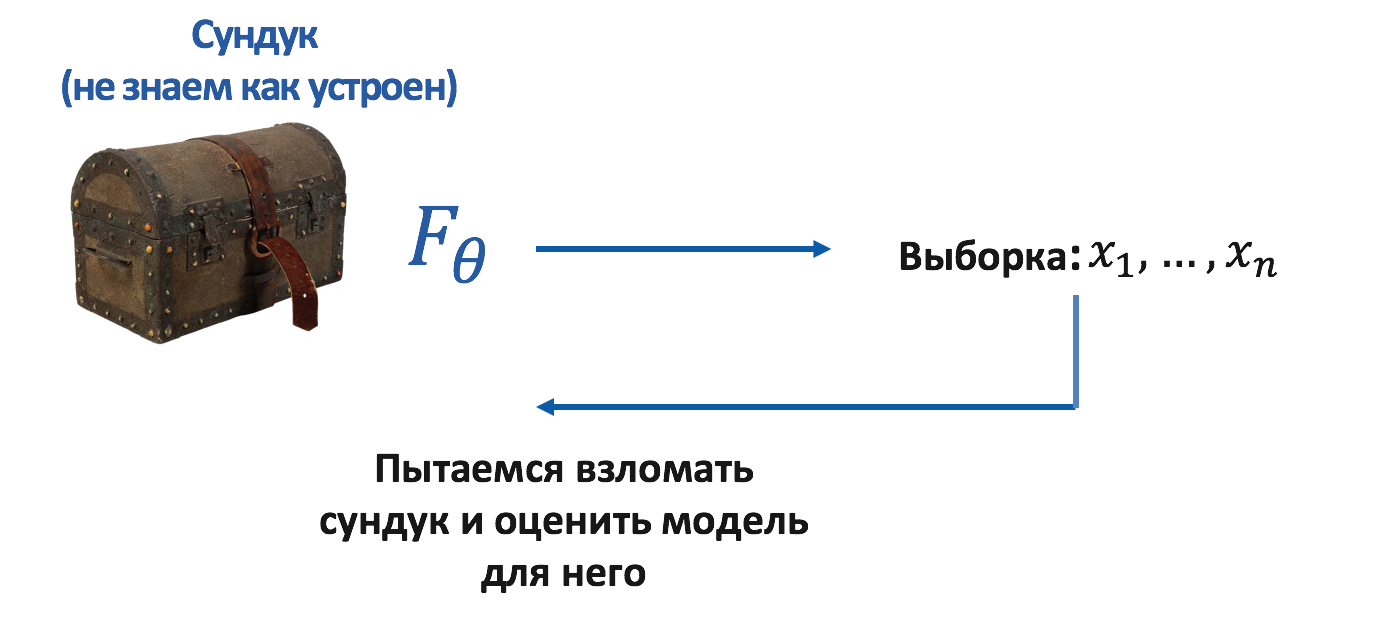
\includegraphics[width=0.8\linewidth]{pic0.png}
\end{center} 

Теория вероятностей занимается тем, что предлагает простейшие модели, которые могли бы описать внутренности сундука. Математическая статистика предлагает кучу способов смотреть на выборки, которые сундук выплюнул. Давайте посмотрим на пару примеров того, как можно формализовать модель, которая бы описывала сундук, и принять какое-то решение на основе данных.

\section{Тест Фишера}

На работу нужно взять $8$ человек. Работодатель говорит, что берёт людей на работу абсолютно беспристрастно. Ему неважно какого пола кандидат. Прособеседовались $20$ человек. Из них $8$ были мужчинами, $12$ женщинами. На работу взяли $7$ мужчин и $1$ женщину. Есть ли на рынке труда дискриминация?  

Мы можем попытаться найти ответ на этот вопрос с помощью данных. Предположения, которые можно проверить с помощью данных, называют \indef{гипотезами.} Нарисуем табличку. Внизу откладываются суммы по столбцам, справа по строкам. Всего собеседовалось $20$ человек. Эту цифру запишем на диагональке. 

\begin{center}
    \begin{tabular}{|r|c|c|c|}
    \hline
                  & мальчик & девочка &        \\ \hline 
         взяли    &   $7$   &   $1$   & $8$    \\ \hline 
         не взяли &   $1$   &   $11$  & $12$   \\ \hline 
                  &   $8$   &   $12$  & $20$   \\ \hline
    \end{tabular}
\end{center}

Допустим, что работодатель не врёт и отбор правда был беспристрастен. Это наш статус-кво. По-другому статус-кво в статистике называют \indef{нулевой гипотезой.} Чтобы отказаться от нулевой гипотезы, нужны весомые доказательства. Какова вероятность получить именно такую выборку, если работодатель не врёт, на рынке нет дискриминации и нулевая гипотеза выполнена?

Всего вариантов выбрать $8$ человек из $20$ существует $C_{20}^8$ способов. Мы взяли $7$ мальчиков и $1$ девочку. Сделать это есть $C_8^7 \cdot C_{12}^1$ способов. Получается, вероятность того, что на $8$ вакансий будет взята только одна девушка составит \[ \frac{C_8^7 \cdot C_{12}^1}{C_{20}^8} \approx 0.00076. \] 

Вероятность того, что всё будет ещё хуже и девушек на работу вообще не возьмут составит \[ \frac{C_8^8 \cdot C_{12}^0}{C_{20}^8} \approx 7 \cdot 10^{-6}. \] 

По аналогии можно посчитать все вероятности для всех возможных комбинаций и нарисовать их на картинке. По оси $x$ отложим число девушек, взятых на работу, по оси $y$ вероятность того, что такая ситуация возможна при беспристрастном отборе, то есть при верности нулевой гипотезы. В сумме все вероятности будут давать единицу. 

\begin{center} 
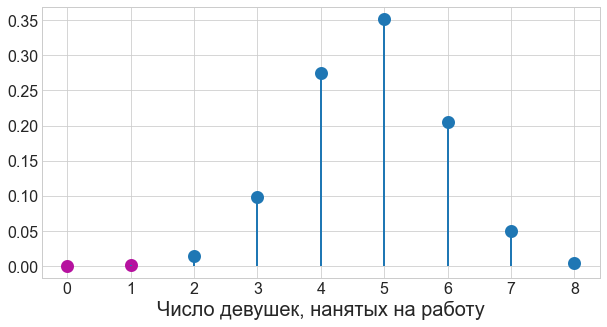
\includegraphics[width=0.7\linewidth]{pic1.png}
\end{center} 

Вероятность того, что при беспристрастном отборе мы увидим нашу ситуацию, либо ситуацию ещё хуже оказывается очень низкой. На картинке исходы, которые соответствуют этому, закрашены лиловым. Вероятность нашего, либо более плохого исхода, при верности нулевой гипотезы, обычно называют  \indef{p-значением (p-value).} Для одной взятой на работу девушки p-значение составляет $0.00077$.

Вероятность оказалась низкой. Это не означает дискриминации на рынке труда, но заставляет нас задуматься. Если нулевая гипотеза верна, и дискриминации нет, то именно такой исход эксперимента, как у нас, должен получаться очень-очень редко. 

Ситуация, в которой на работу берут двух девушек или ещё меньше, при верности нулевой гипотезы, происходит с вероятностью $0.015$. Это уже заметно больше, и при беспристрастном отборе происходит чаще. Если бы результаты нашего эксперимента дали бы три или четыре девушки, взятые на работу, мы бы оказались близко к центру распределения, и никаких вопросов к беспристрастности отбора у нас бы не было. 

К сожалению, в нашей ситуации на работу взяли только одну девушку. Мы анализируем случайную величину --- число девушек взятых на работу. Одна девушка --- это \indef{наблюдаемое значение} нашей случайной величины. Отталкиваясь от него мы должны принять решение, верим ли мы в нулевую гипотезу о беспристрастности. Вопрос в том, как его принять. 

На практике выбирают какое-то место, начиная с которого перестают верить в нулевую гипотезу. Это место называют \indef{критическим значением.} Например, мы можем сказать, что если на работу взяли $2$ девушки и больше, мы верим в беспристрастность. Такая засечка и будет критическим значением, с которым сравнивают значение, полученное в эксперименте. Всё, что левее критического значения, мы считаем аномальным, и отказываемся от нулевой гипотезы. 

Обычно для того, чтобы подобрать критическое значение, перед проведением эксперимента фиксируют \indef{уровень значимости (ошибку первого рода).} Уровень значимости --- это наша готовность ошибаться и зря отказываться от статуса-кво. Если мы возьмём $\alpha = 0.01$, тогда при постоянном повторении эксперимента, мы в $1\%$ случаев ошибочно откажемся от нулевой гипотезы, потому что при беспристрастном отборе такие редкие события иногда происходят. 

Каждому значению $\alpha$ соответствует критическое значение случайной величины. Если мы возьмём $\alpha = 0.01,$ оно будет между $2$ и $1$. Это рубеж для принятия решения. Если на работу взяли две девушки, мы верим в беспристрастность. Если одну, то уже не верим. 

Можно рассуждать о том же самом в терминах $p$-значения. Если оно оказывается большим, фиолетовая площадь на графике оказывается больше, чем уровень значимости, и мы попадаем наблюдаемым значением случайной величины в хорошую зону. Гипотеза не отвергается, мы верим в статус-кво. 

В нашем эксперименте $pvalue = 0.00077$ значение оказалось меньше $\alpha=0.01$. Значит наблюдаемое значение левее критического и от нулевой гипотезы нам надо отказаться. Возможно, что это ошибочное решение. Однако весь смысл этой процедуры заключается в том, что мы хотим мало ошибаться в долгосрочном периоде, при постоянном проведении эксперимента. С $1\%$ ошибок мы согласны смириться. 

Чем меньше $p-$значение, тем аномальнее наши наблюдения. Чем меньше значение уровня значимости, тем в более аномальные наблюдения мы верим. Чем меньше уровень значимости, тем сильнее мы боимся отказаться от нулевой гипотезы, и тем сильнее в хвост распределения углубляется засечка, на основании которой мы принимаем решение. 

Кроме ошибки первого рода, уровня значимости, есть ещё и ошибка второго рода. \indef{Ошибка первого рода ---} это когда мы отказались от нулевой гипотезы (статуса-кво), а она была верна. Вероятность такой ошибки обычно обозначают буквой $\alpha$. \indef{Ошибка второго рода ---} это когда мы остались верны статусу-кво, а он на самом деле неверен. Её вероятность обычно обозначают буквой $\beta$. 

\begin{center}
	\begin{tabular}{|r|c|c|}
	\hline
	                    & $H_0$ верна & $H_0$ не верна \\  \hline 
	выбрали $H_0$       &  ok &    $\beta$ \\      \hline 
	отказались от $H_0$ &   $\alpha$ &  ok \\      \hline 
	\end{tabular}
\end{center}

Ошибка первого и второго рода связаны друг с другом. Когда растёт одна, вторая падает. Жёстко контролировать мы можем только одну из этих ошибок. Вторая минимизируется по остаточному принципу. Для простых критериев можно вывести формулы, которые показывают как эти ошибки связаны друг с другом. Обычно, чем больше собрано данных, тем меньше обе ошибки. В будущем мы научимся такие формулы выводить. 

На практике обычно не хотят отказываться от статуса-кво. Все мысли формулируют именно так, чтобы было сложно от него отказаться. Например, если тестируют какое-то лекарство, намного страшнее выпустить на рынок плохое лекарство, чем не выпустить хорошее. Из-за этого в качестве гипотезы $H_0$ рассматривают ситуацию, когда новое лекарство бесполезно. Нам нужны весомые статистические доказательства, чтобы отказаться от такого статуса-кво. 

Перекос в пользу гипотезы $H_0$ обычно называют \indef{презумпцией нулевой гипотезы.} Это как презумпция невиновности в суде.  Нельзя называть человека убийцей, пока его вина не доказана. Нельзя отказываться от нулевой гипотезы, пока мы не собрали данные и не увидели в них противоречия. Данные --- наш судья. 

Итак, наша нулевая гипотеза --- на рынке нет дискриминации девушек. Альтернативная гипотеза --- дискриминация есть. Если выбрать $\alpha = 0.01$, мы будем вынуждены отвергнуть нулевую гипотезу. Данные говорят против неё. Такую процедуру, которая помогает понять взаимосвязаны ли между собой два дискретных признака называют \indef{тестом Фишера.} В примере выше мы искали взаимосвязь между полом и наймом на работу. 

Выводы, которые мы сделали могут оказаться неверными. Мы действовали в рамках конкретной модели. Когда мы строили тест, мы предполагали что есть только два фактора пол и найм. Вполне возможно, что на самом деле есть какой-то третий признак, который повлиял на эксперимент, а мы его нигде не учли. Возможно, что девушки сами отказались от работы по итогам собеседований, хотя работодатель был готов их взять. 

Когда проводят эксперимент, пытаются исключить все такие третьи факторы из него. Если это оказывается невозможным, либо если эксперимент провести невозможно, приходится привлекать более мощные статистические методы. Модели, описывающие сундук могут быть довольно сложными. При этом не факт, что они тоже хорошо будут описывать реальность.

\section{Критерий знаков}

Мэр сказал в новостях, что больше половины квартир в его городе стоит дешевле $1$~млн. рублей. Как проверить, не врёт ли он? Мы можем собрать случайную выборку из квартир. Целых $n$ штук. Будем ставить $\oplus$, если квартира окажется дешевле $1$~млн. Если квартира будет дороже, будем ставить $\ominus$. 

Мэр не врёт, если плюсиков много. Мы изначально верим ему. Это наш статус-кво, наша нулевая гипотеза. Чтобы отказаться от неё, мы должны увидеть в данных что-то ужасное. Предположим, что мы посмотрели на $10$ квартир. У нас есть $9$ плюсиков и $1$ минусик. Какова вероятность получить такую выборку либо выборку ещё хуже, при верности нулевой гипотезы? 

\begin{center} 
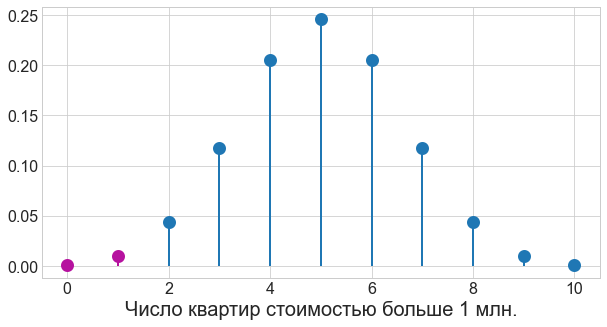
\includegraphics[width=0.7\linewidth]{pic2.png}
\end{center} 

Наш эксперимент представляет из себя неправильную монетку. Если монетка выпала орлом, квартира дешёвая. Если решкой, дорогая. Мы предполагаем, что вероятность орла $p \ge 0.5$. То есть больше половины квартир будут дешёвыми. Альтернатива заключается в том, что $p < 0.5$.  Кратко можно записать это как: 

\begin{equation*} 
    \begin{aligned} 
        &H_0: \quad p \ge 0.5 \\
        &H_a: \quad p < 0.5.
    \end{aligned} 
\end{equation*}

Обычно в таких сложных нулевых гипотезах рассматривают самый шаткий статус-кво. В нашей ситуации таким будет утверждение, что ровно половина квартир оказалась дешевле $1$~млн.

\begin{equation*} 
    \begin{aligned} 
        &H_0: \quad p = 0.5 \\
        &H_a: \quad p < 0.5.
    \end{aligned} 
\end{equation*}

Зафиксируем \indef{уровень значимости} $\alpha = 0.01.$ Мы можем выбирать его любым. Чем меньше мы его возьмём, тем сильнее мы боимся зря отказаться от статуса-кво по ошибке. Ошибки второго рода мы здесь боимся не очень сильно. Лучше ошибочно не назвать мэра лжецом, чем ошибочно назвать. Посчитаем \indef{p-значение,} то есть вероятность получить либо наш исход, либо исход ещё хуже при верности нулевой гипотезы 

\[
pvalue = \frac{10}{2^{10}} + \frac{1}{2^{10}} \approx 0.0107 > \alpha = 0.01.
\]

Получается, что гипотеза о том, что мэр не врёт, не отвергается. Многие скажут, что это противоречит здравому смыслу. И будут правы. На самом деле на такой маленькой выборке, при таком маленьком уровне значимости, ошибка второго рода будет зашкаливать. Чтобы сделать её меньше, не меняя ошибку первого рода, можно собрать более большую выборку. Тогда решение будет более устойчивым. В будущих посиделках мы выведем формулу для ошибки второго рода для данной задачи. 

Такая процедура с расстановкой плюсиков и минусиков называется \indef{критерием знаков}. Её довольно часто используют, когда измерения оказались не очень точными, но при этом нам хочется понять, в какую именно сторону направлены изменения. Например, так довольно часто происходит в биологии. 

Если ваши измерения были сделаны точно, то воспользовавшись критерием знаков, вы потеряете довольно много полезной информации, так как превратите все цифры в единицы и нули. В таких ситуациях лучше использовать другие тесты. Например, в будущем мы будем говорить про тесты для средних, основанные на центральной предельной теореме.  

\section{Ранговый критерий (критерий Манна-Уитни)}

Нам срочно нужно протестировать новое лекарство от гипертонии. Для этого мы воспользуемся \indef{двойным слепым тестированием.} В такой ситуации врач не знает, кому что даёт. Пациент тоже не знает, что именно ему дали. Если врач знает какие таблетки лекарство, а какие плацебо, он пытается давать лекарство тем, кто на его взгляд болен сильнее. Это может исказить результат. Поэтому приходится держать врачей в неведении. 

Вопрос заключается в том, есть ли от лекарства какая-то польза. В качестве статуса-кво выберем гипотезу, что никакой пользы нет. Будем давать лекарство людям из группы $A$. Группе $B$ дадим плацебо. У всех людей измерим давление. 

Разбираться в том, есть ли разница между группами будем с помощью следующей процедуры: свалим все наблюдения в одну кучу и отсортируем их по возрастанию. Каждому наблюдению \indef{припишем свой ранг.} Если все наблюдения разные --- это просто порядковый номер. Если встречаются одинаковые наблюдения, то надо сложить их порядковые номера и поделить на число повторов. 

Например, для выборки $5,-4,5,3,22$ каждому наблюдению будет приписан порядковый номер $3,1,4,2,5$. Третий и четвёртый элементы --- это пятёрки. Если мы хотим превратить порядковые номера в ранги, нужно сложить эти номера и поделить на два. То есть рангами будут числа $3.5, 1, 3.5, 2, 5$.

Пусть в группе $A$ ранги оказались равны $r_1$ и $r_2$. В группе $B$ $r_3, r_4, r_5$. 

\begin{center}
\definecolor{zzttqq}{rgb}{0.6,0.2,0.}
\begin{tikzpicture}[scale=0.8]
\fill[line width=2.pt,color=zzttqq,fill=zzttqq,fill opacity=0.1] (-3.,5.) -- (1.,5.) -- (1.,4.) -- (-3.,4.) -- cycle;
\fill[line width=2.pt,color=zzttqq,fill=zzttqq,fill opacity=0.1] (-3.,3.) -- (3.,3.) -- (3.,2.) -- (-3.,2.) -- cycle;
\draw [line width=2.pt,color=zzttqq] (-3.,5.)-- (1.,5.);
\draw [line width=2.pt,color=zzttqq] (1.,5.)-- (1.,4.);
\draw [line width=2.pt,color=zzttqq] (1.,4.)-- (-3.,4.);
\draw [line width=2.pt,color=zzttqq] (-3.,4.)-- (-3.,5.);
\draw [line width=2.pt,color=zzttqq] (-3.,3.)-- (3.,3.);
\draw [line width=2.pt,color=zzttqq] (3.,3.)-- (3.,2.);
\draw [line width=2.pt,color=zzttqq] (3.,2.)-- (-3.,2.);
\draw [line width=2.pt,color=zzttqq] (-3.,2.)-- (-3.,3.);
\draw (-4,4.8) node[anchor=north west] {\large $A$};
\draw (-4,2.8) node[anchor=north west] {\large $B$};
\draw (-2.5,4.8) node[anchor=north west] {\large $r_1$};
\draw (-0.5,4.8) node[anchor=north west] {\large $r_2$};
\draw (-2.5,2.8) node[anchor=north west] {\large $r_3$};
\draw (-0.5,2.8) node[anchor=north west] {\large $r_4$};
\draw (1.5,2.8) node[anchor=north west] {\large $r_5$};
\draw [line width=2.pt,color=zzttqq] (-1.,5.)-- (-1.,4.);
\draw [line width=2.pt,color=zzttqq] (-1.,3.)-- (-1,2);
\draw [line width=2.pt,color=zzttqq] (1.,3.)-- (1,2);
\end{tikzpicture}
\end{center}

Если получается так, что сумма $r_1 + r_2$ оказалась маленькой, это сигнализирует нам о том, что лекарство помогает, и давление понижается. Как понять, как будет распределена такая статистика? 

Предположим, что все наши наблюдения разные. Тогда ранги принимают значения $1,2,3,4,5$. Самое маленькое значение для $r_1 + r_2$ будет равно $1 + 2 = 3.$ Самое большое $5 + 4 = 9$. Посчитаем вероятность того, что $r_1 + r_2 = 6.$ Всего два числа из пяти можно выбрать $C_5^2 = 10$ способами. В сумме $6$ можно получить двумя способами. Получается, что $\PP(r_1 + r_2 = 6) = 0.2$. По аналогии можно посчитать все другие вероятности. 

\begin{center} 
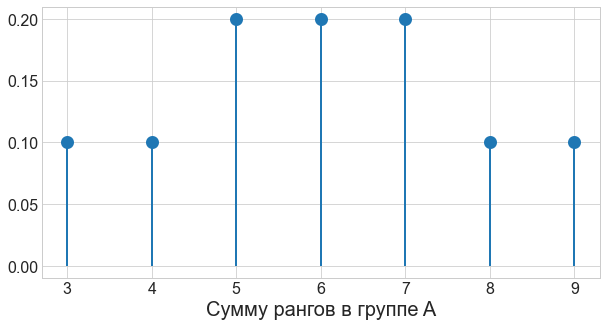
\includegraphics[width=0.7\linewidth]{pic3.png}
\end{center} 

Осталось понять, насколько наша ситуация плохая и принять решение в соответствии с тем уровнем значимости, который мы выбрали до начала эксперимента. 

Обратите внимание, что в этой задачке мы впервые явно выписали случайную величину, на основе которой мы принимаем решение. Это $T = r_1 + r_2$. В первых двух пунктах можно также выписать такую случайную величину. Для критерия знаков --- это число плюсов. Для критерия Фишера --- это число нанятых девушек. 

Каждый раз мы принимаем решение на основе того, как эта случайная величина себя ведёт при верности нулевой гипотезы. Если она показывает аномальные значения, мы не верим в нулевую гипотезу. Такие случайные величины называют \indef{статистиками.} 

Принимая решение мы можем рассуждать как в терминах уровня значимости и $p$-значения, так и в терминах \indef{наблюдаемого значения статистики и критического значения статистики.}   Наблюдаемое значение рассчитывается по выборке, критическое получается исходя из уровня значимости. Если наблюдаемое значение слишком далеко от центра распределения, данные говорят против статуса-кво. Критическое значение --- это порог, начиная с которого мы прекращаем верить в нулевую гипотезу.

Для данной ситуации нам надо найти такое значение $T$, левее которого лежит $\alpha$ процентов распределения. Это значение и будет критическим. 

Многие статистические процедуры можно построить отталкиваясь от таких статистик,  случайных величин --- помощников. Самое главное --- знать их распределения при статусе-кво, при верности нулевой гипотезы. Есть разные теоремы, которые нам эти распределения подсказывают. Во всех трёх рассмотренных критериях нам не понадобилось каких-то особенных теорем. Мы смогли выписать все распределения в явном виде благодаря простой комбинаторике. 

Критерий, который мы описали выше, обычно называют \indef{критерием рангов.} В нём мы точно также отказываемся от изначальных измерений, предполагая что они не очень точные. Но в отличие от критерия знаков, мы пытаемся сохранить чуть больше информации, используя вместо плюсов и минусов, порядковые номера измерений.


\section{Схема статистики}

Любое исследование в анализе данных происходит примерно по одной и той же схеме. Сначала у нас есть \indef{вопросы.} Мы хотим найти на них ответы. Нас могут интересовать дискриминация, изменение цен, работоспособность лекарств и многое многое другое. 

Чтобы грамотно ответить на каждый из этих вопросов, нужно собрать данные. Для этого мы проводим \indef{эксперимент.} Эксперименты нужно планировать аккуратно. Продумыванию условий эксперимента в статистике уделяется особое внимание. Выборка, которая получается в результате его проведения, должна быть \indef{репрезентативной.} То есть она должна отражать те свойства, которые действительно присущи всей \indef{генеральной совокупности.} В ходе эксперимента мы собираем \indef{данные.} 

Сундук выплюнул на нас данные. Пора выяснить что именно внутри сундука. Нужно предположить как именно устроен мир вокруг нас, то есть надо придумать какую-то \indef{модель.} Любая модель работает только в той ситуации, когда выполнены все её предпосылки. Про них нельзя забывать. В будущих посиделках мы постоянно будем обращать внимание на предпосылки и разбираться с тем, как их можно проверить. 

\begin{center}
\begin{tikzpicture}[scale=1.4]
	\tikzstyle{place}=[draw=black, minimum height=25pt,minimum width=60pt,inner sep=2pt]
	
    \draw node at (0, 1.5) (q) {\Large \textbf Вопрос};
    \draw node at (1.2, 1.5) {\Large $\Rightarrow$};
    \draw node at (3, 1.5) (e) {\Large \textbf Эксперимент};

	\draw node at (1.3, 0.6) (data) {\Large $x_1, \ldots, x_n  \quad \sim  \quad F_{\theta}$};
	\draw node at (0.4, 0.1) {\textbf{Данные}};
	\draw node at (2.7, 0.1) {\textbf{Модель}};
\end{tikzpicture}
\end{center}   	
    	
С помощью собранных данных мы можем \indef{оценить неизвестные параметры $\theta$} нашей модели $F_{\theta}$.	Есть довольно много методов для оценки. В будущем мы будем обсуждать каждый из них более подробно. Оценки неизвестных параметров обычно отмечают колпачком. Так $\hat{\theta}$ --- это оценка неизвестного параметра $\theta$. 

Когда у нас есть готовая оценка, нам хочется понимать насколько точной она получилась. Для этого надо знать как она распределена, то есть нужно найти её плотность распределения $f_{\hat \theta} (t)$. Тут к нам на помощь будут приходить разные \indef{союзники --- теоремы.} Это может быть центральная предельная теорема или какие-то специфические распределения вроде распределения Стьюдента.

На основе распределения оценки $\hat \theta$ мы можем проверять гипотезы и строить доверительные интервалы, то есть пытаться понять насколько наша оценка получилась точной. 

Например, в трёх критериях выше, мы пользовались дискретными распределениями, которые мы выводили с помощью простейшей комбинаторики. Она была нашим союзником. Никакие параметры в этих распределениях нам оценивать не надо было, достаточно было просто посчитать вероятности.

Тем не менее, эти критерии очень простые и они игнорируют довольно много информации из выборки. Они слишком упрощают её. Чем больше у модели параметров, тем лучше она может описать данные и тем качественнее может получится ответ на мучающий нас вопрос. Если конечно мы не \indef{переобучимся.} Переобучением называют ситуацию, когда модель вместо того, чтобы обобщить данные, запомнила их. Чем больше у модели параметров, тем легче ей переобучиться. 


\begin{center}
    \begin{tikzpicture}[scale = 1.5, line cap=round,line join=round,x=1.0cm,y=1.0cm]
    
        \path (-1,0) node(x) {\Huge $\hat \theta$} (3,0) node(y) {\Huge $f_{\hat \theta} (t)$};
        
        \node at (8, 0) {\footnotesize
            \begin{varwidth}{\linewidth}\begin{itemize}
                \item прогнозы
                \item насколько точны прогнозы
                \item ответы на вопросы (гипотезы)
            \end{itemize}\end{varwidth}
        };
        
        \draw[->, line width=1.1pt] (-0.5,0) -- (2,0);
        \draw[->, line width=1.1pt] (4,0) -- (6,0);
        
        \node at (0.8, 1.6) { \footnotesize
            \begin{varwidth}{\linewidth} \textbf{Хотим:}
            \begin{itemize}
                \item несмещённость
                \item состоятельность
                \item эффективность
            \end{itemize}\end{varwidth}
        };
    
        \node at (-0.2, -1.45) { \footnotesize
            \begin{varwidth}{\linewidth} \textbf{Cоюзники:}
            \begin{itemize}
                \item метод моментов
                \item метод максимального \\ правдоподобия
            \end{itemize}\end{varwidth}
        };
        
        \node at (3.5, -1.7) { \footnotesize
            \begin{varwidth}{\linewidth} \textbf{Cоюзники:}
            \begin{itemize}
                \item ЦПТ
                \item Дельта-метод
                \item $\chi^2_n, t(n), F(n,m)$
                \item Теорема Фишера
            \end{itemize}\end{varwidth}
        };
    \end{tikzpicture}
\end{center} 

Ещё нам часто будет хотеться, чтобы оценки неизвестных параметров обладали хорошими свойствами: \indef{немещённостью, состоятельностью и эффективностью.} Методы оценивания придумывают так, чтобы добиваться этих свойств.  

Отдельно хочется обратить внимание на то, что идти по схеме матстата можно очень по-разному. Можно отталкиваться от средних и строить всю науку через закон больших чисел и центральную придельную теорему. Можно использовать метод максимального правдоподобия и его свойства. Можно предположить, что параметр $\theta$ на самом деле какая-то случайная величина и пойти по дороге байесовской статистики. Можно пойди по дороге информационных подходов. 

Обо всём этом мы будем подробно разговаривать в следующих посиделках. В следующей мы на простом примере введём ещё несколько понятий и построим наш первый доверительный интервал. 
\end{document}
